\begin{frame}{Comparación de preferencias}
\begin{alertblock}{Ordenador usado para la ejecuci\'on}
	Asus N56VJ

	Sistema operativo: Linux mint (Rosa)

	Memoria: 8GB

	Procesador: Inter Core i7-4710HQ x 8

	Gráficos: Nvidia geforce 750M

	Tipo de SO: 64 bits

	Disco: 1TB
	\end{alertblock}
\end{frame}

\subsection{Problema}
\begin{frame}{Problema}
	\begin{block}{Explicación}
	Queremos comparar las preferencias de dos personas sobre un número n de productos (películas, musica, ...). Para ello contaremos el número de inversiones en su valoración de los productos.\\
	Consideramos que una valoración está invertida cuando A prefiere el producto j antes que i y B prefiere el producto i antes que j. 
	\end{block}
	
	\begin{block}{Simplificación}
		\begin{table}
		\begin{tabular}{|c|c|c|c|c|c|c|c|c|c|c|c|}
		Obj & A & B & & Obj & A & B & & A & B & & v\\
		1 & 3 & 2 & & 3 & 3 & 2 & & 1 & 3 & & 3\\
		2 & 1 & 3 & & 1 & 1 & 3 & & 2 & 1 & & 1\\
		3 & 2 & 1 & & 2 & 2 & 1 & & 3 & 2 & & 2\\
		\end{tabular}
		\end{table}
	\end{block}
	
\end{frame}

\subsection{Fuerza bruta}
\begin{frame}{Fuerza bruta}
	\begin{columns}
		
		\begin{column}{4cm}
		\begin{block}{Algoritmo}
		La aproximación más básica al problema es comprobar en cada elemento si los siguientes en el vector son menores.\\
		\end{block}	
		
		\begin{block}{Criterio}
		Dos elementos están invertidos si $i < j$ pero $v[i] > v[j]$\\
		\end{block}	
		\end{column}
		\pause
			
		\begin{column}{6.5cm}
		\begin{exampleblock}{Implementación}
		\lstinputlisting[language=C++, firstline=10, lastline=19]{../Opcional/src/fuerza_bruta.cpp}
		\end{exampleblock}
		\end{column}
		
	\end{columns}
\end{frame}

\begin{frame}{Eficiencia}
\begin{columns}
	\begin{column}{5cm}
	\begin{block}{Eficiencia teórica}
	$$T(n) = \sum_{i=1}^{n-1}n-i$$
	$$T(n) = \frac{n^2 - n}{2} \longrightarrow O(n^2)$$
	\end{block}
	
	\begin{block}{Ajuste}
		$a = 4.62037 \cdot 10^{-9}$\\ $b = 7.56764 \cdot 10^{-9}$\\ $c = -3.85366 \cdot 10^{-5}$
	\end{block}
	\end{column}
	
	\begin{column}{6.5cm}
	\begin{figure}[h]
	\centering
		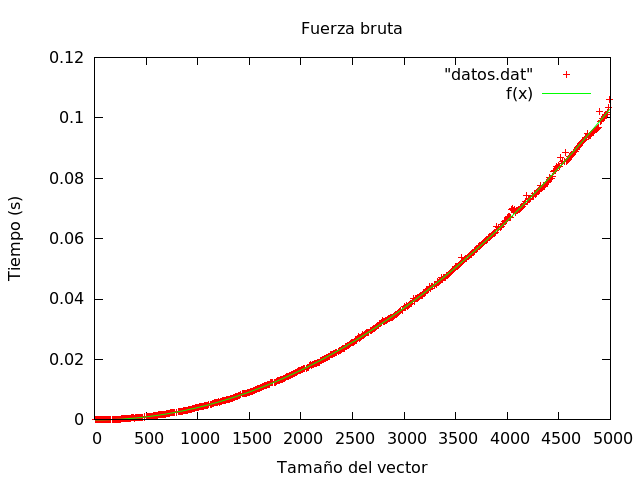
\includegraphics[width=1\textwidth]{../Opcional/Graficas/fuerza_bruta_bruno.png}
	\end{figure}
	\end{column}
\end{columns}
\end{frame}


\subsection{Divide y vencerás}
\begin{frame}{Divide y vencerás}
	\begin{columns}
		
		\begin{column}{4cm}
		\begin{block}{Algoritmo}
		Utilizamos el método de mezcla para contar el número de inversiones en cada sección.\\
		\end{block}	
		
		\begin{block}{Criterio}
		Dos elementos están invertidos si $i < j$ pero $v[i] > v[j]$\\
		\end{block}	
		\end{column}
			
		\begin{column}{6cm}
		\begin{exampleblock}{Ejemplo}
		\begin{figure}[h]
			\centering
			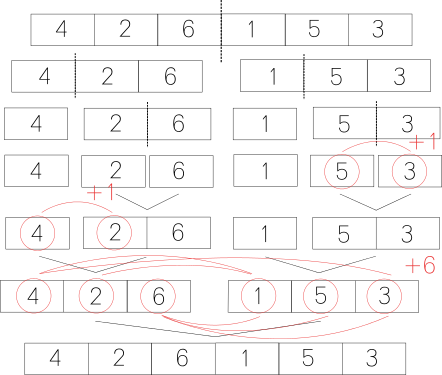
\includegraphics[width=1\textwidth]{Imagenes/esquema.png}
		\end{figure}
		\end{exampleblock}
		\end{column}
		
	\end{columns}
\end{frame}

\begin{frame}{Implementación}
\lstinputlisting[language=C++, firstline=112, lastline=128]{../Opcional/src/dyv.cpp}
\end{frame}

\begin{frame}{Eficiencia teórica}
\begin{block}{Recurrencia}
$$\left\lbrace
	\begin{array}{l}
	T(n) = \frac{n^2 - n}{2}\  si\ n \leq 2\\
	T(n) = 2T(\frac{n}{2}) + 2n\  si\ n > 2 \\
	\end{array}
	\right.$$\\
\end{block}

\begin{block}{Solución}
$$n=2^k \Rightarrow k = \log_2n$$
$$T(k) = 2^kT(1) + 2^kn$$
$$T(n) = n \cdot 0 + n^2$$
$$O(n^2)$$
\end{block}
\end{frame}

\begin{frame}{Eficiencia empírica}
\begin{figure}[h]
	\centering
		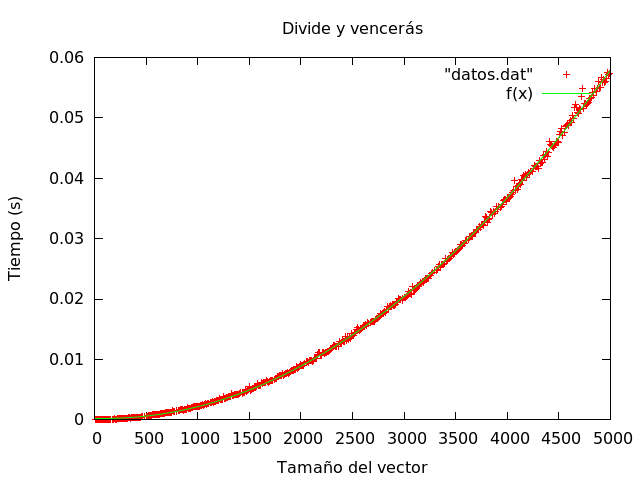
\includegraphics[width=0.6\textwidth]{../Opcional/Graficas/dyv_bruno.png}
\end{figure}

\begin{block}{Ajuste}
\begin{center}
$a = 2.6999 \cdot 10^{-9}$
$b = -8.47849 \cdot 10^{-7}$
$c = 0.000424603$
\end{center}
\end{block}
\end{frame}


\subsection{Divide y vencerás con mergesort}
\begin{frame}{Divide y vencerás con mergesort}
	\begin{columns}
		
		\begin{column}{4cm}
		\begin{block}{Algoritmo}
		Utilizamos el algoritmo de ordenación mergesort para contar el número de inversiones.\\
		\end{block}	
		
		\begin{block}{Criterio}
		Dos elementos están invertidos si $i < j$ pero $v[i] > v[j]$\\
		\end{block}	
		\end{column}
			
		\begin{column}{6cm}
		\begin{exampleblock}{Ejemplo}
		\begin{figure}[h]
			\centering
			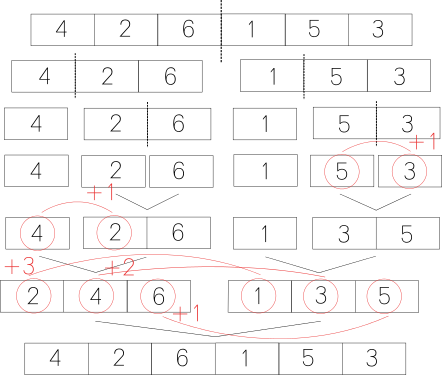
\includegraphics[width=1\textwidth]{Imagenes/esquema_merge.png}
		\end{figure}
		\end{exampleblock}
		\end{column}
		
	\end{columns}
\end{frame}

\begin{frame}{Implementación}
\lstinputlisting[language=C++, firstline=111, lastline=128]{../Opcional/src/dyv_mergesort.cpp}
\end{frame}

\begin{frame}{Eficiencia}
\begin{columns}
\begin{column}{5cm}
\begin{block}{Eficiencia teórica}
Tiene la misma eficiencia que mergesort, $O(n\log n)$
\end{block}

\begin{block}{Ajuste}
$a = 1.99872 \cdot 10^{-8}$
\end{block}
\end{column}

\begin{column}{6.5cm}
\begin{figure}[h]
	\centering
	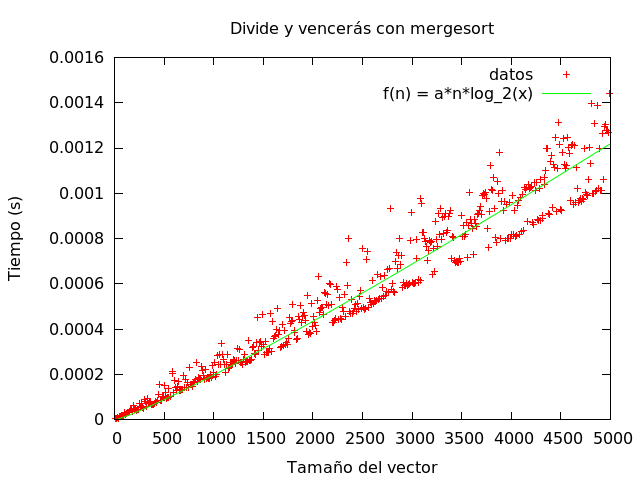
\includegraphics[width=1\textwidth]{../Opcional/Graficas/dyv_mergesort_bruno.png}
\end{figure}
\end{column}
\end{columns}
\end{frame}

\subsection{Comparación}
\begin{frame}{Comparación}
\begin{exampleblock}{Tabla comparativa}
\begin{table}
\begin{tabular}{|l|l|l|l|}
\multicolumn{1}{c}{\textbf{N}} & \multicolumn{1}{c}{\textbf{FUERZA BRUTA}} & \multicolumn{1}{c}{\textbf{DyV}} & \multicolumn{1}{c}{\textbf{MERGESORT}} \\
\hline
10                                                     & 5.372e-06                                                         & 5.01e-06                                                 & 4.475e-06                                                          \\
\hline
100                                                    & 4.3868e-05                                                        & 4.5584e-05                                               & 1.7295e-05                                                         \\
\hline
500                                                    & 0.00113                                                           & 0.000778726                                              & 8.8503e-05                                                         \\
\hline
1000                                                   & 0.0045925                                                         & 0.00247251                                               & 0.000218733                                                        \\
\hline
1500                                                   & 0.0106898                                                         & 0.00567031                                               & 0.000289624                                                        \\
\hline
2000                                                   & 0.0171023                                                         & 0.0094678                                                & 0.000382864                                                        \\
\hline
\end{tabular}
\end{table}
\end{exampleblock}
\end{frame}

\begin{frame}
\begin{figure}[h]
	\centering
	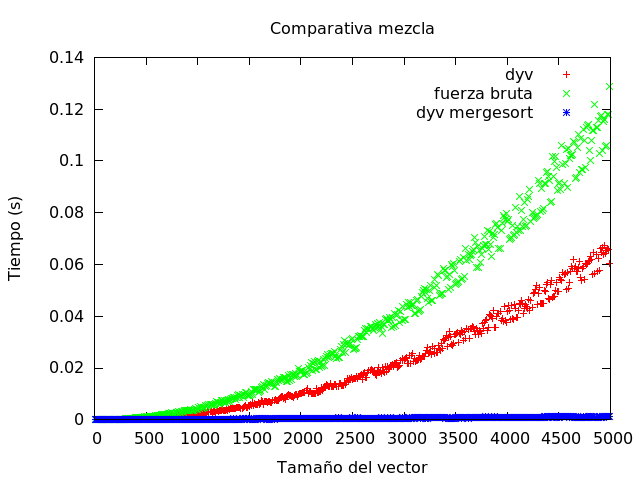
\includegraphics[width=1\textwidth]{../Opcional/Graficas/comparativa.png}
\end{figure}
\end{frame}